\documentclass[11pt]{article}
\usepackage{csc512}

%%%%%%%%%%%%%%%%%%%% name/id
\rfoot{\small Brian Park | 200190057}


%%%%%%%%%%%%%%%%%%%% Course/HW info
\newcommand*{\instr}{Xu Liu}
\newcommand*{\term}{Fall 2022}
\newcommand*{\coursenum}{CSC 512}
\newcommand*{\coursename}{Compiler Construction}
\newcommand*{\hwnum}{0}

\rhead{\LARGE   \fontfamily{lmdh}\selectfont	Project \hwnum}

\lfoot{\small \coursenum, \term, Project \hwnum}

%%%%%%%%%%%%%%%%%%%%%%%%%%%%%% Document Start %%%%%%%%%%%%%%%%%
\begin{document}

%%%%%%%%%%%%%%%%%%%%%%%%%%%%%%%%%%%%%%%%%%%%%%%%%%%%%%%%%%%%%%%%%%%%%%%%%%%%%%%%%%%%%%%%
% Question 1
%%%%%%%%%%%%%%%%%%%%%%%%%%%%%%%%%%%%%%%%%%%%%%%%%%%%%%%%%%%%%%%%%%%%%%%%%%%%%%%%%%%%%%%%
\Question{Build DrCCTProf and Run the Example Clients}
\centerline{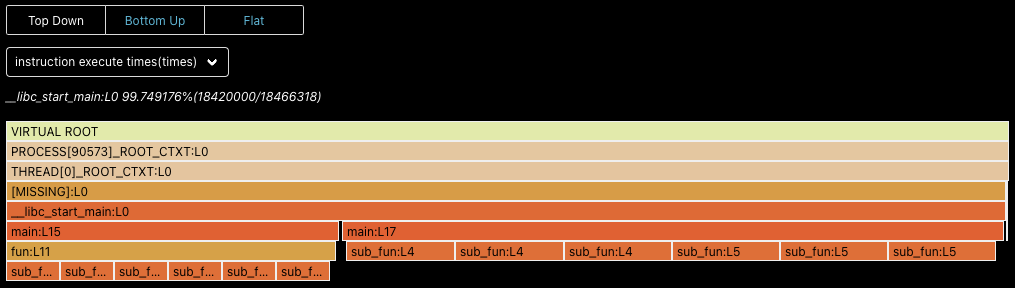
\includegraphics[width=6in]{figures/easyview.png}}

Output of EasyView provides detailed call stack of the functions called. Next to the function name includes the line number from the source code that the function name was called from. This is useful in profiling a specific subroutine. Hovering over a specific block will output the percentage spent in overall runtime of the function. It seems to capture everything before a program is run, up to creating a process/thread and to executing \verb|libc_start_main|.

\Question{Write Your Own Client Tool}

\end{document}